This Section explains the method and principles used for the system used for the system evaluation process, measuring and comparing the performance (latency, in seconds, and throughput, in rows/second) of reading and writing Hudi, Iceberg and Delta Lake tables on \gls{HopsFS}. Those operations are conducted respectively on the current legacy system, on the newly integrated PyIceberg-based system and on the Rust-based system, implemented in related work \cite{manfrediReducingReadWrite2024}.

\subsection{Evaluation process - RQ1}
\label{subsec:eval_process}
The evaluation process will follow a sequential approach described in Figure~\ref{fig:method_experiments}. Each step of this process is related to one of the \glspl{G}~3-6 associated with the \gls{RQ}~1 in Section \ref{sec:intro_goals}, to which this process partially answer. The relationships between each process activity and \glspl{G} are here explained:
\begin{enumerate}
    \item \textbf{Design experiments}: this activity maps perfectly to \gls{G}~3, designing the experiments that will be conducted to evaluate the performance difference in performance between the current legacy access to Apache Hudi compared to the PyIceberg library-based access to Icbeerg Tables in \gls{HopsFS}. 
    \item \textbf{Perform experiments}: this activity maps perfectly to \gls{G}~4, using the integration detail (\gls{D}3-partial) to develop and conduct the designed experiments on the analyzed systems. Here, data is collected as latency, expressed in seconds.
    \item \textbf{Transform data according to metrics}: this activity is requisite to fulfill \gls{G}~5, and \gls{G}~8 of \gls{RQ}~2. The activity is conducted because throughput is not directly measured, but it is computed from latency following the formula here below:
    \[ Throughput \; (rows/second) = \frac{Number \; of \; rows \; (rows)}{Latency \;(seconds)}\]
    \item \textbf{Visualize results}: this activity maps perfectly to \gls{G}~5, visualizing the experiments' result according latency, measured in seconds, and throughput, measured in rows/second. This activity also generates \gls{D}~1, the experiment results complemented with tables and histograms, presented in Chapter \ref{ch:results_and_analysis}.
    \item \textbf{Analyze results}: this activity maps perfectly to \gls{G}~6, analyzing and interpreting the results delivered in D2. This deliverable contributes to D3, generating the analysis of results, i.e., Chapter \ref{ch:results_and_analysis}.
\end{enumerate}
\begin{figure}[!ht]
    \begin{center}
    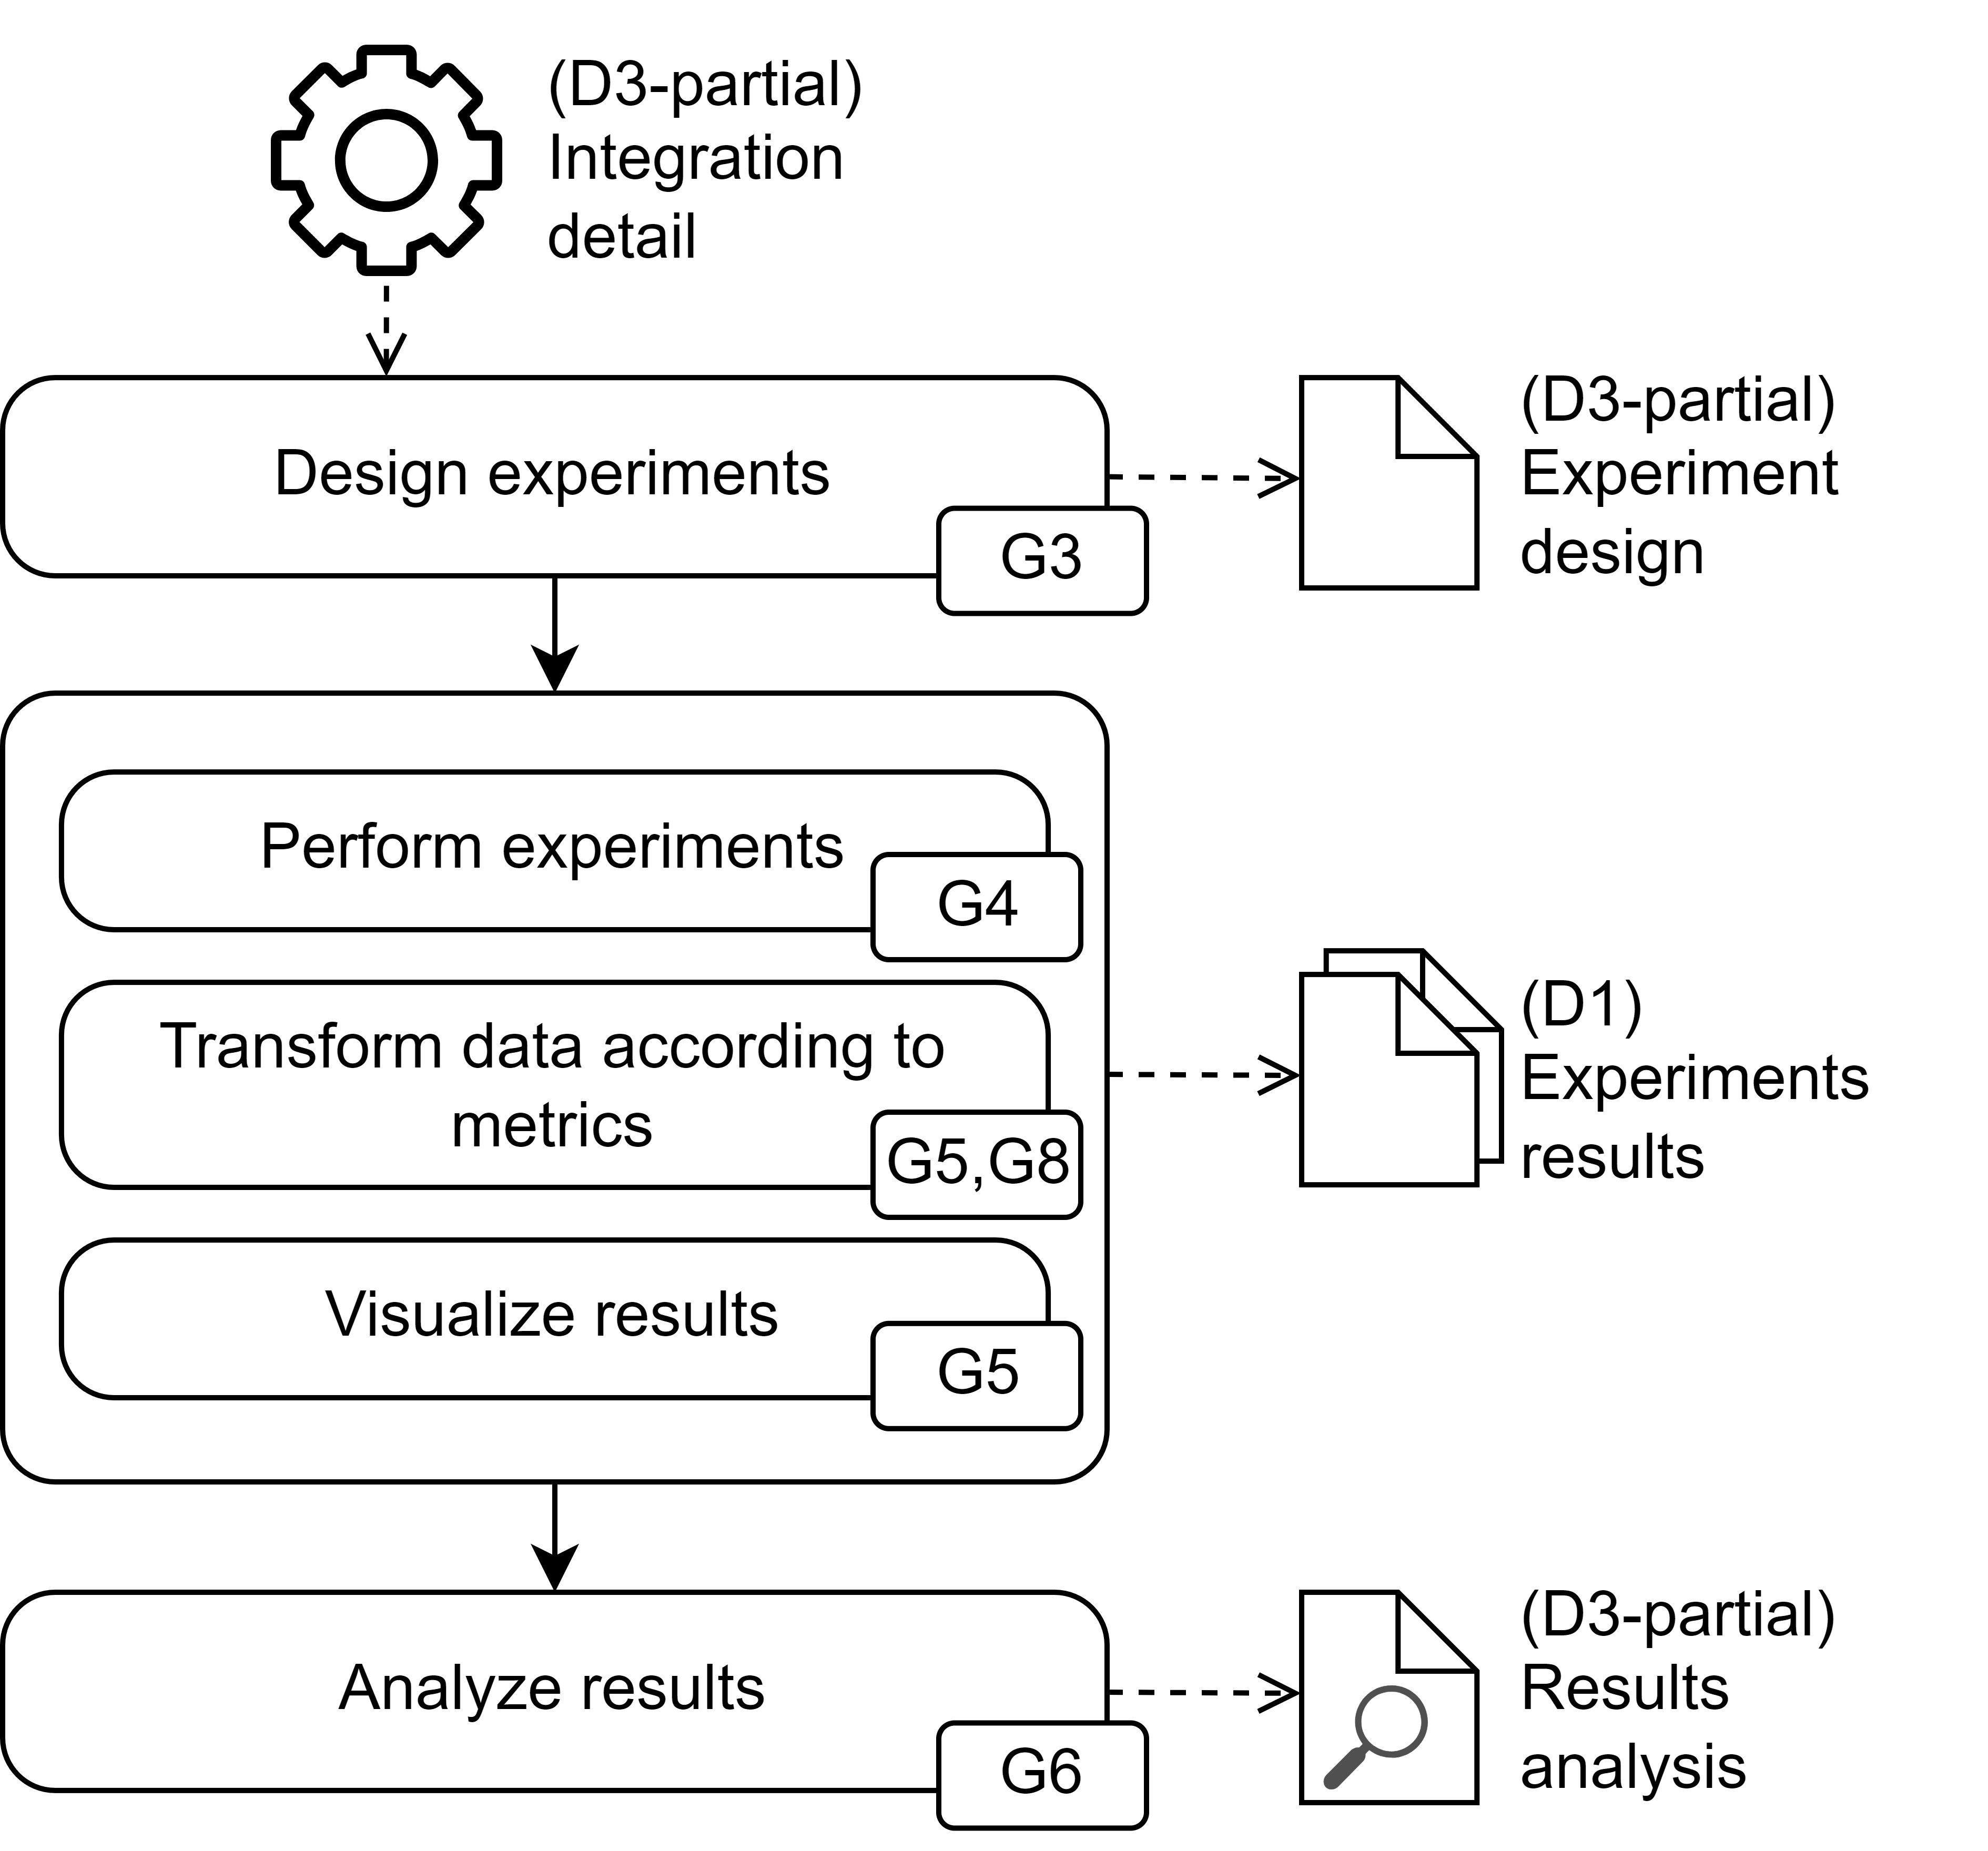
\includegraphics[width=\textwidth]{figures/3-method/method_exp.png}
    \caption[System evaluation process]{Diagram of the system evaluation process partially answering \gls{RQ}~1. Each activity is associated to specific \gls{G}. The process produces two \glspl{D}, the experiments results (\gls{D}~1) and a results analysis (\gls{D}3-partial).}
    \label{fig:method_experiments}
    \end{center}
\end{figure}